\documentclass{standalone}
\usepackage{tikz}
\usetikzlibrary{patterns, positioning}

\begin{document}
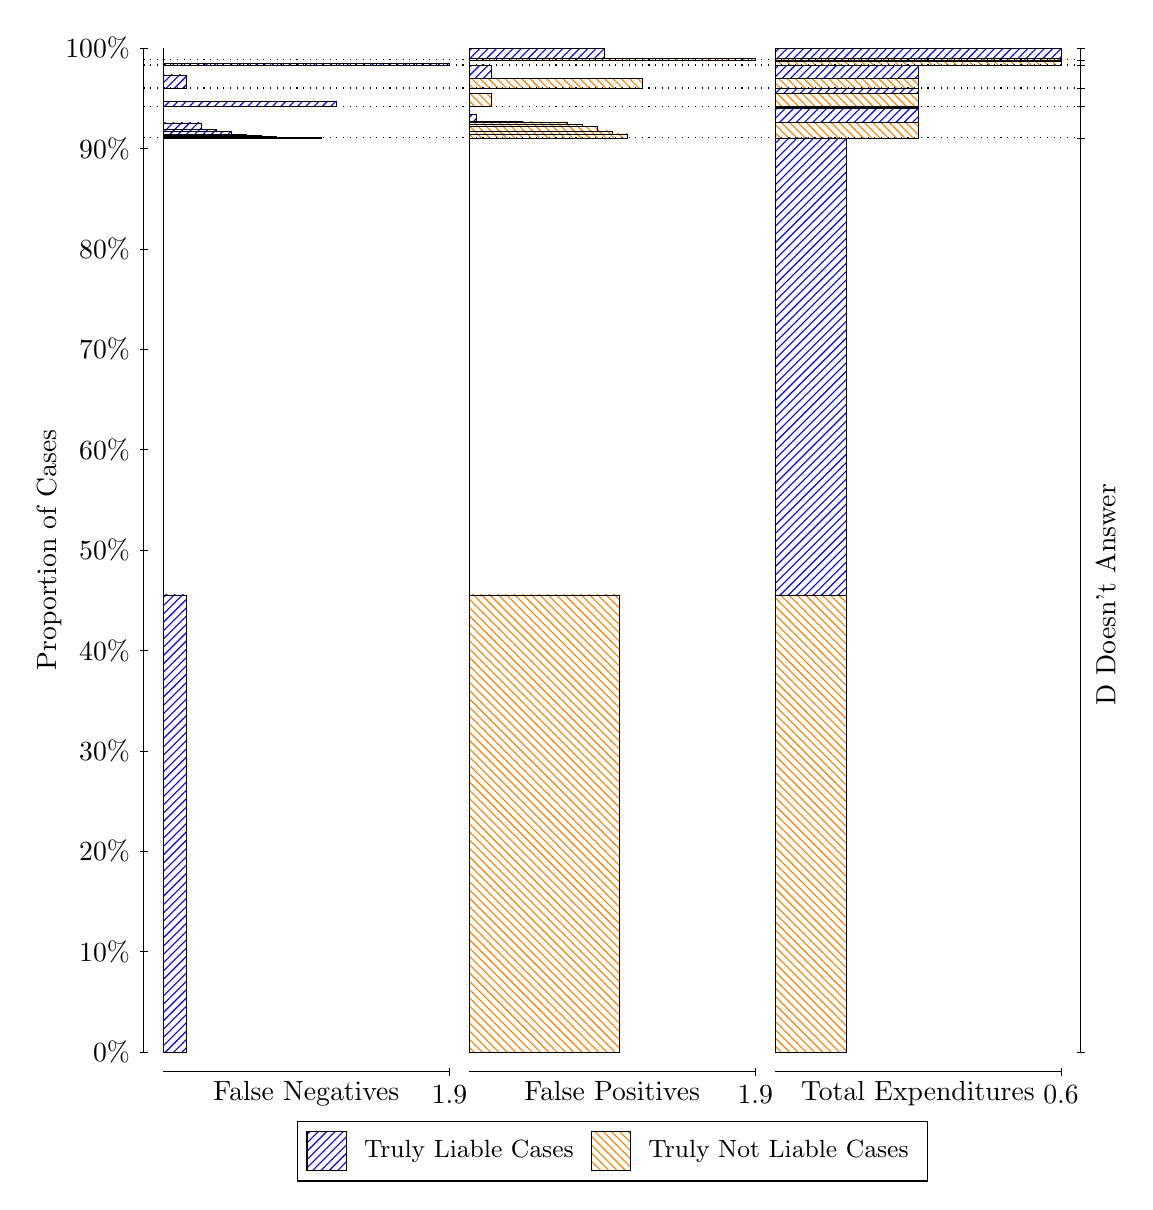
\begin{tikzpicture}
\draw[black, very thin] (1.5,1.75) -- (1.5,14.5);
\node[rotate=90, anchor=center] at (0.3, 8.125) {Proportion of Cases};
\draw[black, very thin] (1.45,1.75) -- (1.55,1.75);
\node[anchor=east] at (1.45, 1.75) {0\%};
\draw[black, very thin] (1.45,3.025) -- (1.55,3.025);
\node[anchor=east] at (1.45, 3.025) {10\%};
\draw[black, very thin] (1.45,4.3) -- (1.55,4.3);
\node[anchor=east] at (1.45, 4.3) {20\%};
\draw[black, very thin] (1.45,5.575) -- (1.55,5.575);
\node[anchor=east] at (1.45, 5.575) {30\%};
\draw[black, very thin] (1.45,6.85) -- (1.55,6.85);
\node[anchor=east] at (1.45, 6.85) {40\%};
\draw[black, very thin] (1.45,8.125) -- (1.55,8.125);
\node[anchor=east] at (1.45, 8.125) {50\%};
\draw[black, very thin] (1.45,9.4) -- (1.55,9.4);
\node[anchor=east] at (1.45, 9.4) {60\%};
\draw[black, very thin] (1.45,10.675) -- (1.55,10.675);
\node[anchor=east] at (1.45, 10.675) {70\%};
\draw[black, very thin] (1.45,11.95) -- (1.55,11.95);
\node[anchor=east] at (1.45, 11.95) {80\%};
\draw[black, very thin] (1.45,13.225) -- (1.55,13.225);
\node[anchor=east] at (1.45, 13.225) {90\%};
\draw[black, very thin] (1.45,14.5) -- (1.55,14.5);
\node[anchor=east] at (1.45, 14.5) {100\%};

\draw[black, very thin] (13.4,1.75) -- (13.4,14.5);
\draw[black, very thin] (13.35,1.75) -- (13.45,1.75);
\node[anchor=west] at (13.35, 1.75) {};
\draw[black, very thin] (13.35,13.359) -- (13.45,13.359);
\node[anchor=west] at (13.35, 13.359) {};
\draw[black, very thin] (13.35,13.758) -- (13.45,13.758);
\node[anchor=west] at (13.35, 13.758) {};
\draw[black, very thin] (13.35,13.992) -- (13.45,13.992);
\node[anchor=west] at (13.35, 13.992) {};
\draw[black, very thin] (13.35,14.284) -- (13.45,14.284);
\node[anchor=west] at (13.35, 14.284) {};
\draw[black, very thin] (13.35,14.35) -- (13.45,14.35);
\node[anchor=west] at (13.35, 14.35) {};
\draw[black, very thin] (13.35,14.5) -- (13.45,14.5);
\node[anchor=west] at (13.35, 14.5) {};

\draw[black, very thin, pattern color=blue, pattern=north east lines] (1.75,1.75) rectangle (2.0368,7.5543);
\draw[black, very thin, pattern color=orange, pattern=north west lines] (1.75,7.5543) rectangle (1.75,13.359);
\draw[black, very thin, pattern color=blue, pattern=north east lines] (1.75,13.359) rectangle (3.7579,13.362);
\draw[black, very thin, pattern color=blue, pattern=north east lines] (1.75,13.362) rectangle (3.5667,13.364);
\draw[black, very thin, pattern color=blue, pattern=north east lines] (1.75,13.364) rectangle (3.3754,13.37);
\draw[black, very thin, pattern color=blue, pattern=north east lines] (1.75,13.37) rectangle (3.1842,13.376);
\draw[black, very thin, pattern color=blue, pattern=north east lines] (1.75,13.376) rectangle (2.993,13.391);
\draw[black, very thin, pattern color=blue, pattern=north east lines] (1.75,13.391) rectangle (2.8018,13.405);
\draw[black, very thin, pattern color=blue, pattern=north east lines] (1.75,13.405) rectangle (2.6105,13.439);
\draw[black, very thin, pattern color=blue, pattern=north east lines] (1.75,13.439) rectangle (2.4193,13.464);
\draw[black, very thin, pattern color=blue, pattern=north east lines] (1.75,13.464) rectangle (2.2281,13.548);
\draw[black, very thin, pattern color=orange, pattern=north west lines] (1.75,13.548) rectangle (1.75,13.758);
\draw[black, very thin, pattern color=blue, pattern=north east lines] (1.75,13.758) rectangle (3.9491,13.822);
\draw[black, very thin, pattern color=orange, pattern=north west lines] (1.75,13.822) rectangle (1.75,13.992);
\draw[black, very thin, pattern color=blue, pattern=north east lines] (1.75,13.992) rectangle (2.0368,14.159);
\draw[black, very thin, pattern color=orange, pattern=north west lines] (1.75,14.159) rectangle (1.75,14.284);
\draw[black, very thin, pattern color=blue, pattern=north east lines] (1.75,14.284) rectangle (5.3833,14.305);
\draw[black, very thin, pattern color=orange, pattern=north west lines] (1.75,14.305) rectangle (1.75,14.35);
\draw[black, very thin, pattern color=orange, pattern=north west lines] (1.75,14.35) rectangle (1.75,14.372);
\draw[black, very thin, pattern color=blue, pattern=north east lines] (1.75,14.372) rectangle (1.75,14.5);
\draw[black, very thin, pattern color=orange, pattern=north west lines] (5.6333,1.75) rectangle (7.5456,7.5545);
\draw[black, very thin, pattern color=blue, pattern=north east lines] (5.6333,7.5545) rectangle (5.6333,13.359);
\draw[black, very thin, pattern color=orange, pattern=north west lines] (5.6333,13.359) rectangle (7.6412,13.411);
\draw[black, very thin, pattern color=orange, pattern=north west lines] (5.6333,13.411) rectangle (7.45,13.447);
\draw[black, very thin, pattern color=orange, pattern=north west lines] (5.6333,13.447) rectangle (7.2588,13.506);
\draw[black, very thin, pattern color=orange, pattern=north west lines] (5.6333,13.506) rectangle (7.0675,13.529);
\draw[black, very thin, pattern color=orange, pattern=north west lines] (5.6333,13.529) rectangle (6.8763,13.552);
\draw[black, very thin, pattern color=orange, pattern=north west lines] (5.6333,13.552) rectangle (6.6851,13.555);
\draw[black, very thin, pattern color=orange, pattern=north west lines] (5.6333,13.555) rectangle (6.6851,13.558);
\draw[black, very thin, pattern color=orange, pattern=north west lines] (5.6333,13.558) rectangle (6.4939,13.563);
\draw[black, very thin, pattern color=orange, pattern=north west lines] (5.6333,13.563) rectangle (6.3026,13.566);
\draw[black, very thin, pattern color=orange, pattern=north west lines] (5.6333,13.566) rectangle (6.1114,13.568);
\draw[black, very thin, pattern color=blue, pattern=north east lines] (5.6333,13.568) rectangle (5.7289,13.653);
\draw[black, very thin, pattern color=blue, pattern=north east lines] (5.6333,13.653) rectangle (5.6333,13.758);
\draw[black, very thin, pattern color=orange, pattern=north west lines] (5.6333,13.758) rectangle (5.9202,13.927);
\draw[black, very thin, pattern color=blue, pattern=north east lines] (5.6333,13.927) rectangle (5.6333,13.992);
\draw[black, very thin, pattern color=orange, pattern=north west lines] (5.6333,13.992) rectangle (7.8325,14.116);
\draw[black, very thin, pattern color=blue, pattern=north east lines] (5.6333,14.116) rectangle (5.9202,14.284);
\draw[black, very thin, pattern color=orange, pattern=north west lines] (5.6333,14.284) rectangle (5.6333,14.329);
\draw[black, very thin, pattern color=blue, pattern=north east lines] (5.6333,14.329) rectangle (5.6333,14.35);
\draw[black, very thin, pattern color=orange, pattern=north west lines] (5.6333,14.35) rectangle (9.2667,14.372);
\draw[black, very thin, pattern color=blue, pattern=north east lines] (5.6333,14.372) rectangle (7.3544,14.5);
\draw[black, very thin, pattern color=orange, pattern=north west lines] (9.5167,1.75) rectangle (10.425,7.5545);
\draw[black, very thin, pattern color=blue, pattern=north east lines] (9.5167,7.5545) rectangle (10.425,13.359);
\draw[black, very thin, pattern color=orange, pattern=north west lines] (9.5167,13.359) rectangle (11.333,13.555);
\draw[black, very thin, pattern color=blue, pattern=north east lines] (9.5167,13.555) rectangle (11.333,13.73);
\draw[black, very thin, pattern color=orange, pattern=north west lines] (9.5167,13.73) rectangle (11.333,13.733);
\draw[black, very thin, pattern color=blue, pattern=north east lines] (9.5167,13.733) rectangle (11.333,13.736);
\draw[black, very thin, pattern color=orange, pattern=north west lines] (9.5167,13.736) rectangle (11.333,13.746);
\draw[black, very thin, pattern color=blue, pattern=north east lines] (9.5167,13.746) rectangle (11.333,13.758);
\draw[black, very thin, pattern color=orange, pattern=north west lines] (9.5167,13.758) rectangle (11.333,13.927);
\draw[black, very thin, pattern color=blue, pattern=north east lines] (9.5167,13.927) rectangle (11.333,13.992);
\draw[black, very thin, pattern color=orange, pattern=north west lines] (9.5167,13.992) rectangle (11.333,14.116);
\draw[black, very thin, pattern color=blue, pattern=north east lines] (9.5167,14.116) rectangle (11.333,14.284);
\draw[black, very thin, pattern color=orange, pattern=north west lines] (9.5167,14.284) rectangle (13.15,14.329);
\draw[black, very thin, pattern color=blue, pattern=north east lines] (9.5167,14.329) rectangle (13.15,14.35);
\draw[black, very thin, pattern color=orange, pattern=north west lines] (9.5167,14.35) rectangle (13.15,14.372);
\draw[black, very thin, pattern color=blue, pattern=north east lines] (9.5167,14.372) rectangle (13.15,14.5);
\draw[black, dotted] (1.5,13.359) -- (13.4,13.359);
\draw[black, dotted] (1.5,13.758) -- (13.4,13.758);
\draw[black, dotted] (1.5,13.992) -- (13.4,13.992);
\draw[black, dotted] (1.5,14.284) -- (13.4,14.284);
\draw[black, dotted] (1.5,14.35) -- (13.4,14.35);
\draw[black, very thin] (1.75,1.5) -- (5.3833,1.5);
\node[anchor=north] at (3.5667, 1.5) {False Negatives};
\draw[black, very thin] (5.3833,1.45) -- (5.3833,1.55);
\node[anchor=north] at (5.3833, 1.45) {1.9};

\draw[black, very thin] (5.6333,1.5) -- (9.2667,1.5);
\node[anchor=north] at (7.45, 1.5) {False Positives};
\draw[black, very thin] (9.2667,1.45) -- (9.2667,1.55);
\node[anchor=north] at (9.2667, 1.45) {1.9};

\draw[black, very thin] (9.5167,1.5) -- (13.15,1.5);
\node[anchor=north] at (11.333, 1.5) {Total Expenditures};
\draw[black, very thin] (13.15,1.45) -- (13.15,1.55);
\node[anchor=north] at (13.15, 1.45) {0.6};

\node[black, centered, rotate=90] at (13.72, 7.5544) {D Doesn't Answer};






\draw (7.449999999999999,1.5) node[draw=none] (baseCoordinate) {};
\begin{scope}[align=center]
        \matrix[scale=0.5, draw=black, below=0.5cm of baseCoordinate, nodes={draw}, column sep=0.1cm]{
            \node[rectangle, draw, minimum width=0.5cm, minimum height=0.5cm, pattern=north east lines, pattern color=blue] {}; &
            \node[draw=none, font=\small] (B) {Truly Liable Cases}; &
            \node[rectangle, draw, minimum width=0.5cm, minimum height=0.5cm, pattern=north west lines, pattern color=orange] {}; &
            \node[draw=none, font=\small] (B) {Truly Not Liable Cases}; \\
            };
\end{scope}

\end{tikzpicture}
\end{document}